\section{Plano de trabalho}
Tendo em conta a dimensão da aplicação foi criado um plano de trabalho onde mapeámos as tarefas
de desenvolvimento no tempo de forma contínua tornado assim possível adaptar um ritmo de trabalho
consistente com os prazos de entrega de cada fase e então cumprir as metas do projecto.
Nesse sentido dividimos o projecto em três fases, sendo elas o planeamento e análise de requisitos, o
desenvolvimento e a documentação.
No que diz respeito à fase de planeamento e análise de requisitos, esta fase engloba todo o levantamento 
de funcionalidades assim como todo o planeamento e estruturação do projecto como
criação do modelo de domínio, diagramaa de classes, modelação do repositório de dados,
análise da concorrência, plano tecnológico, etc.
Para esta fase de planeamento, análise e modelação foi criado um plano de um mês onde todas as tarefas 
teriam de estar concluídas. Na imagem seguinte é possível ver um diagrama de Gannt com
o planeamento inicial.



\begin{figure}[htbp] 
	\centering
	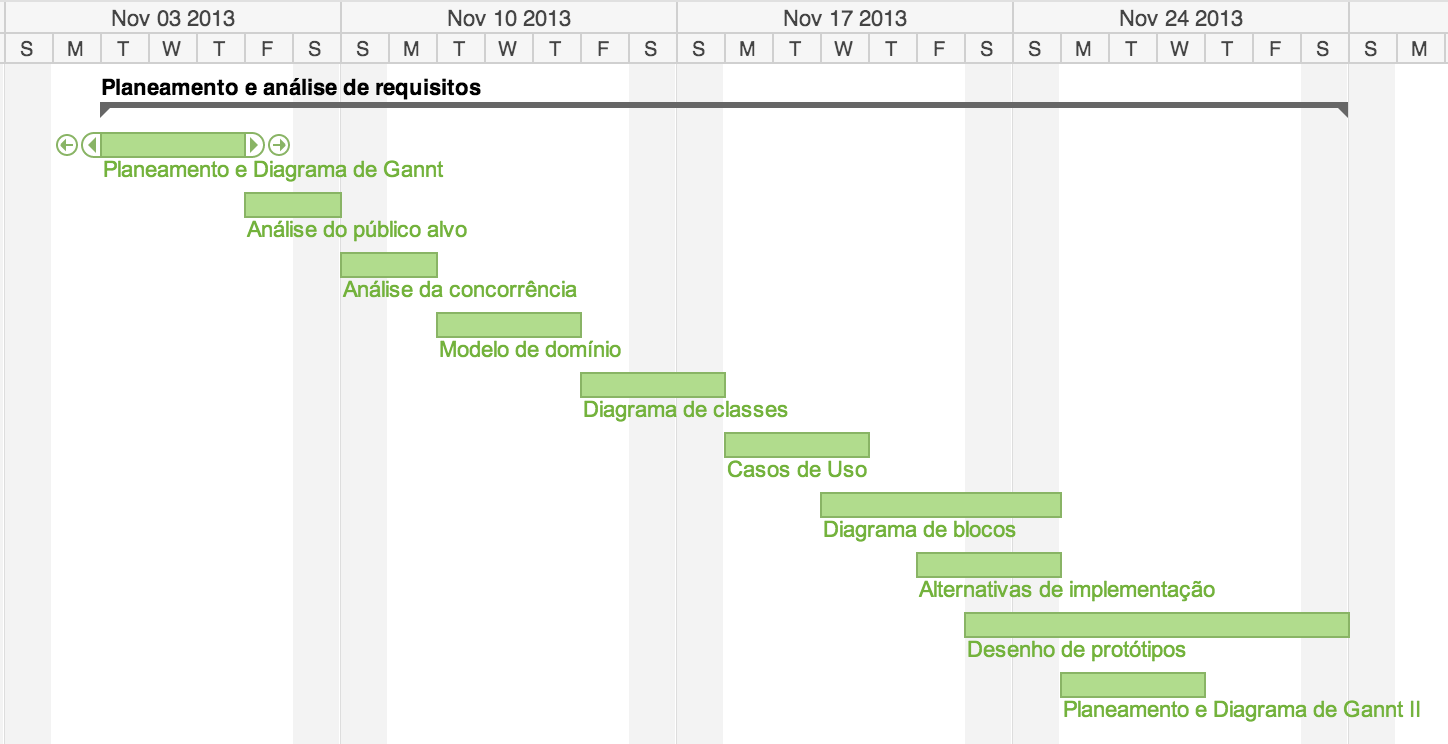
\includegraphics[width=1\textwidth]{images/plano_trabalho_1.png}
 	\caption{Diagrama de Gannt para o planeamento e análise de requisitos}
 	\label{fig: workplan1}
\end{figure}


De seguida, prosseguindo para o planeamento da fase de desenvolvimento após 
analisar as funcionalidades e modelar o sistema  é altura de começar a 
prototipar a aplicação e começar a iterar sobre as funcionalidades a 
implementar. Neste sentido englobámos aqui tarefas como prototipagem em HTML, 
criação de migrações na modelação da base dados, modelação das entidades a 
representar (modelos) na forma da arquitectura MVC seguindo-se a implementação dos 
controladores e visões tendo como base as funcionalidades a desenvolver para o 
sistema.  Nesta fase pretende-se tornar a aplicação capaz de suportar os seus 
utilizadores (não registados, docentes e alunos) das tarefas de gestão de UCs, 
projectos, grupos, submissões, assim como consulta e disponibilização de 
projectos. De forma a tornar a aplicação o mais robusta possível planeamos um 
espaço temporal dedicado a testes de usabilidade e funcionalidade de forma a 
corrigir todos os pormenores que possam ter um impacto negativo.


\begin{figure}[htbp] 
	\centering
	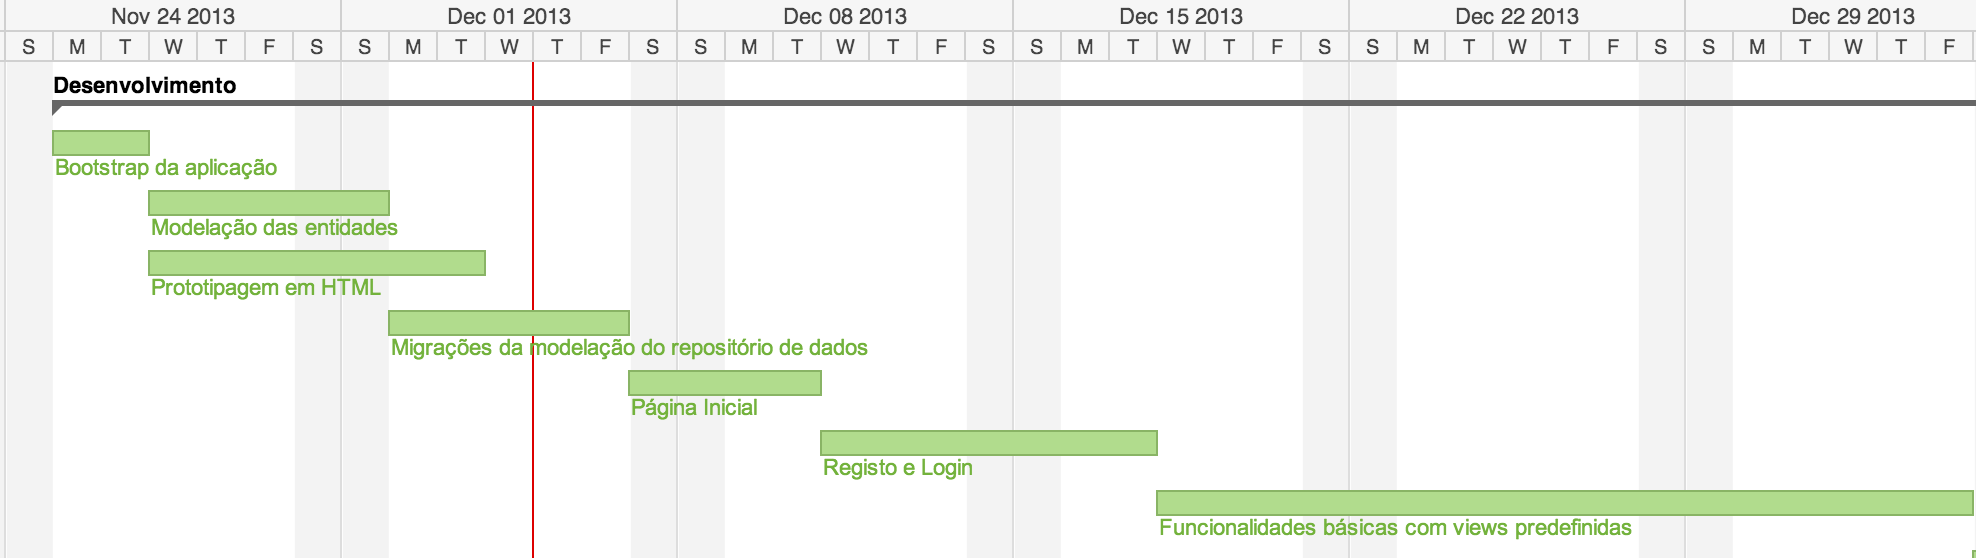
\includegraphics[width=1\textwidth]{images/plano_trabalho_2.png}
 	\caption{Diagrama de Gannt para o desenvolvimento I}
 	\label{fig: workplan2}
\end{figure}

\begin{figure}[htbp] 
	\centering
	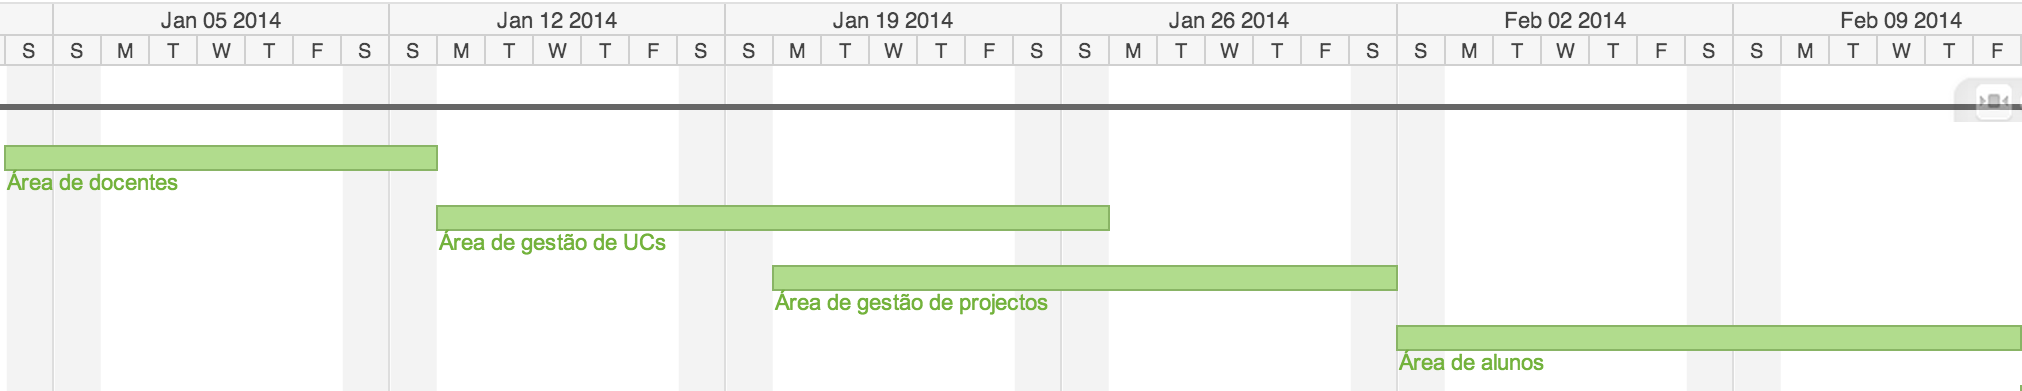
\includegraphics[width=1\textwidth]{images/plano_trabalho_3.png}
 	\caption{Diagrama de Gannt para o desenvolvimento II}
 	\label{fig: workplan3}
\end{figure}

\begin{figure}[htbp] 
	\centering
	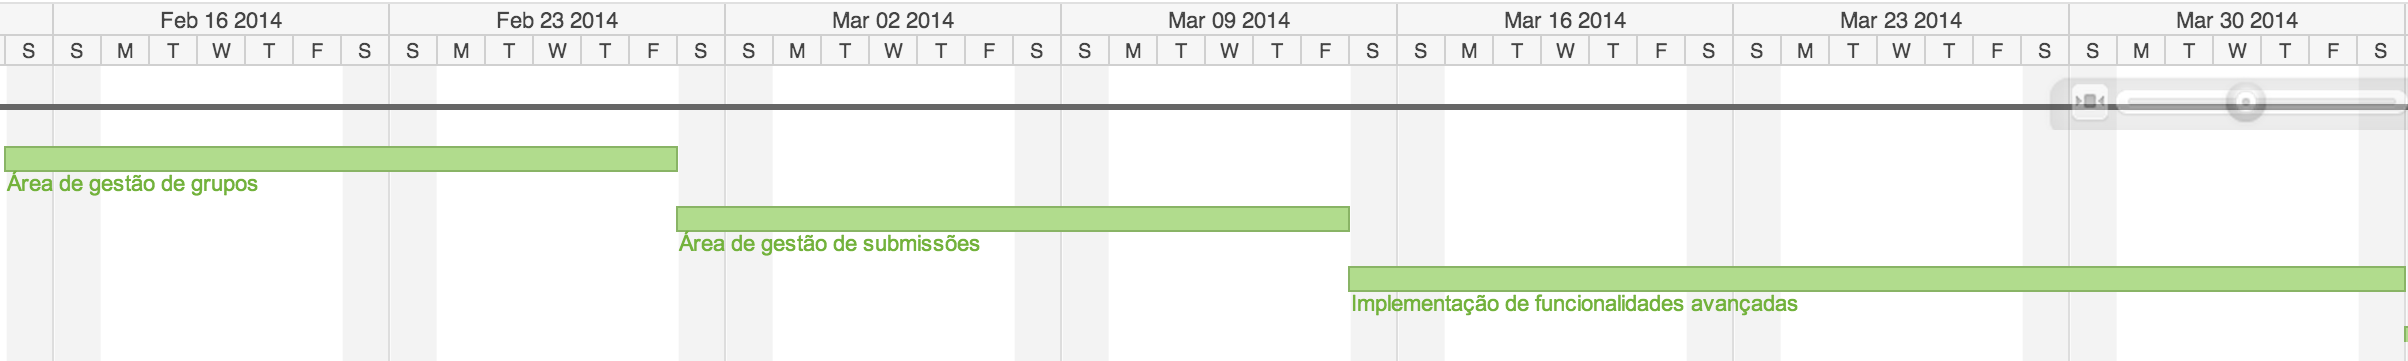
\includegraphics[width=1\textwidth]{images/plano_trabalho_4.png}
 	\caption{Diagrama de Gannt para o desenvolvimento III}
 	\label{fig: workplan4}
\end{figure}

\begin{figure}[htbp!] 
	\centering
	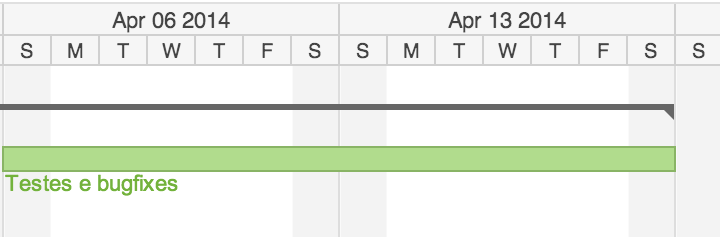
\includegraphics[width=1\textwidth]{images/plano_trabalho_5.png}
 	\caption{Diagrama de Gannt para o desenvolvimento IV}
 	\label{fig: workplan5}
\end{figure}


Por fim, terminámos com a fase de documentação onde será feita toda a descrição 
do sistema desenvolvido em termos de funcionalidades e implementação de forma a 
possibilitar a consulta tanto aos interessados em utilizar a aplicação bem como 
de forma a suportar a possível necessidade de manutenção da aplicação. Desta 
forma qualquer um pode entender todo o sistema na sua plenitude através da 
documentação criada. Para esta fase reservou-se o restante tempo disponível até 
à entrega final do projecto.

